\section{Question 2}

\subsection{Question}
\verbatiminput{q2/q2.txt}

\subsection{Answer}
The ascii and jpeg dendrograms were created using the method shown in Listing \ref{listing:clust:main}, which is modeled after the example from class. 

\lstinputlisting[language=Python, caption={creating the dendrograms}, label=listing:clust:main,linerange={286-293},firstnumber=286]{q2/clusters.py}

This uses the {\tt readfile} function shown in Listing \ref{listing:clust:read} to read the data that was compiled from Question 1 into the script where it is then processed by the {\tt hcluster} function found in Listing \ref{listing:clust:hclust} to produce the clustered representation of the blogs.

\lstinputlisting[language=Python, caption={creating the dendrograms}, label=listing:clust:read,linerange={3-16},firstnumber=3]{q2/clusters.py}

\lstinputlisting[language=Python, caption={hcluster function}, label=listing:clust:hclust,linerange={48-88},firstnumber=48]{q2/clusters.py}

The {\tt printclust} function from Listing \ref{listing:clust:printclust} prints the ascii dendrogram of the cluster object parameter.

\lstinputlisting[language=Python, caption={printclust function}, label=listing:clust:printclust,linerange={90-103},firstnumber=90]{q2/clusters.py}

The {\tt drawdendrogram} function from Listing \ref{listing:clust:drawdendro} creates a jpeg image of the cluster, which is shown in Figure \ref{fig:clust}.

\lstinputlisting[language=Python, caption={drawdendrogram function}, label=listing:clust:drawdendro,linerange={122-139},firstnumber=122]{q2/clusters.py}

\begin{figure}[h!]
\centering
\fbox{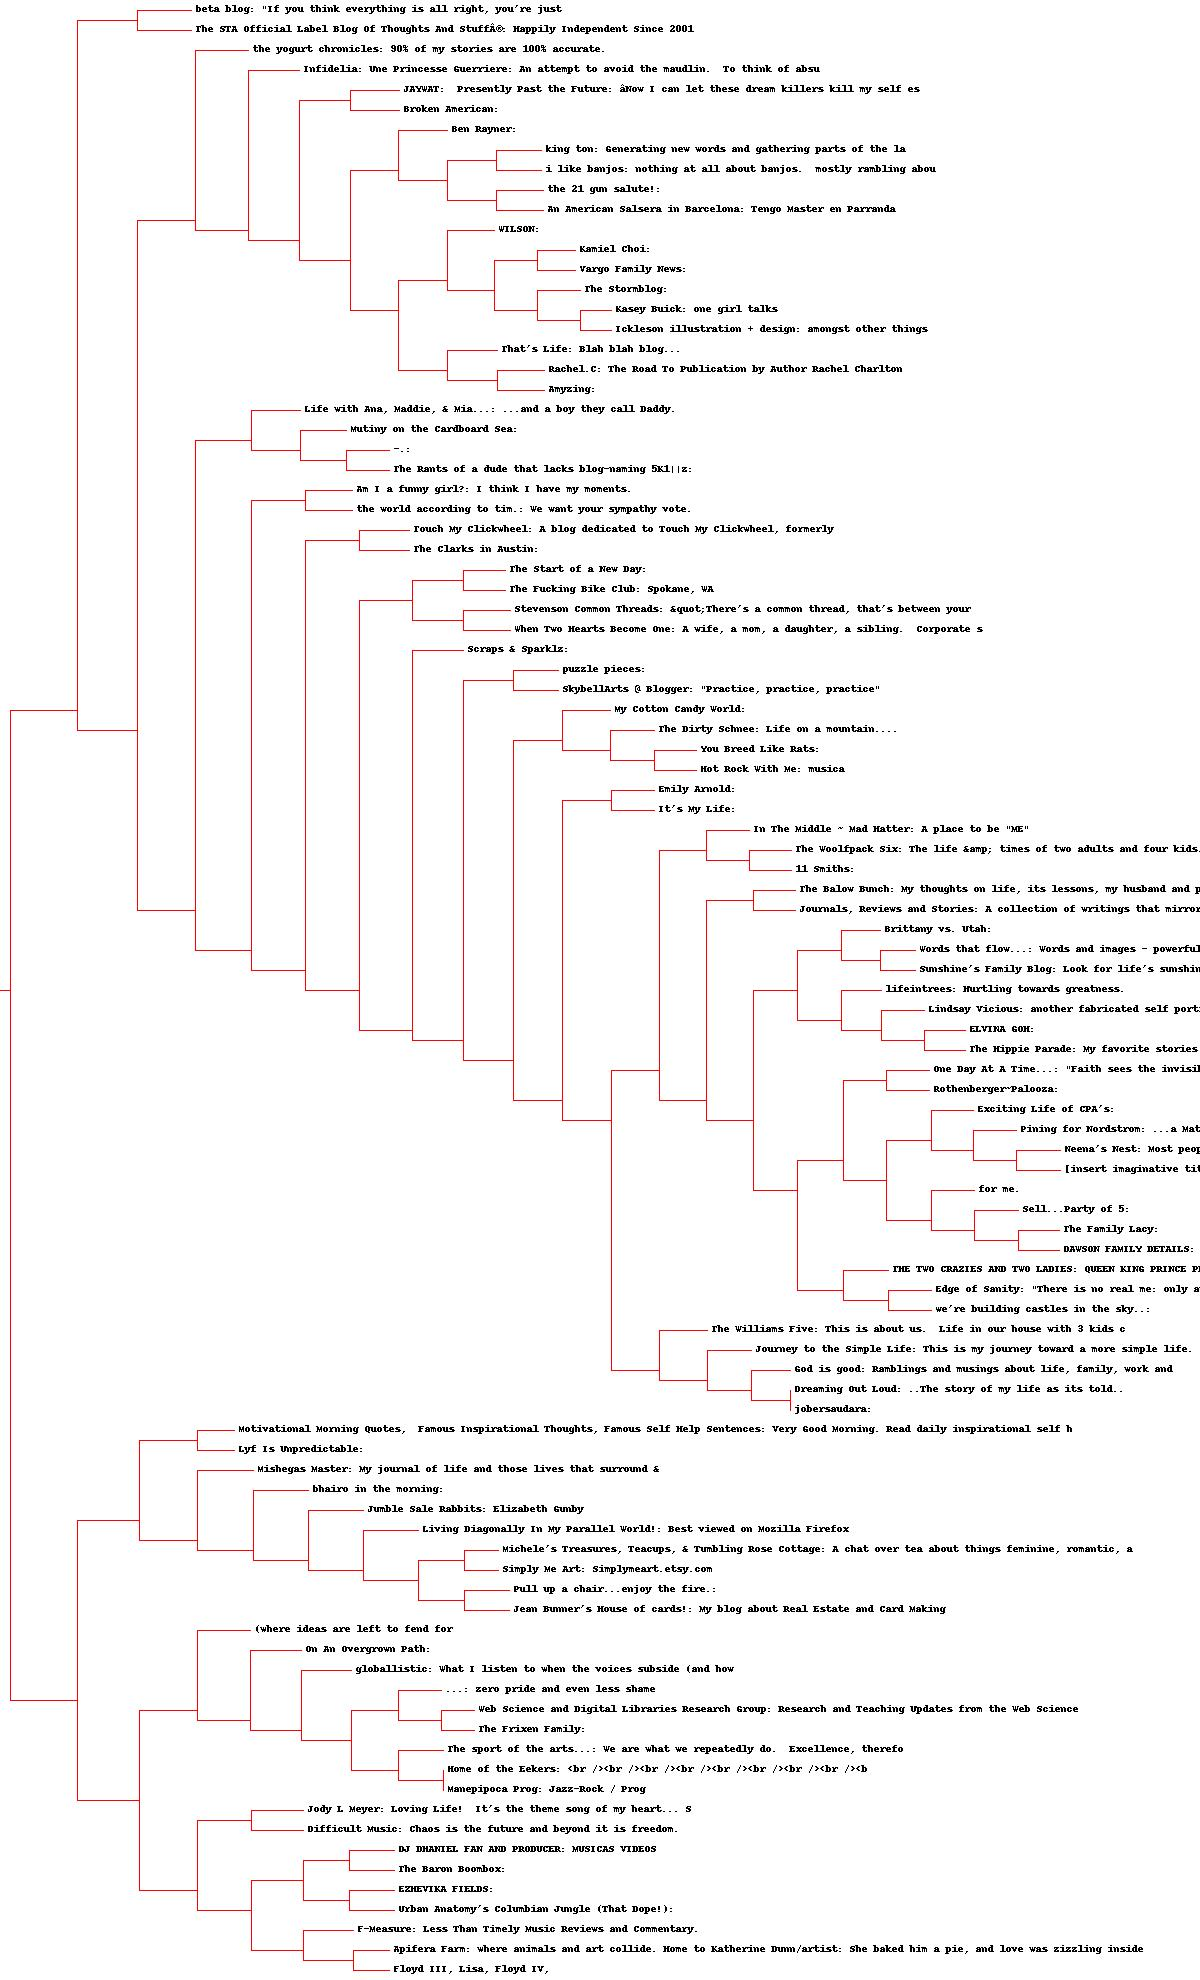
\includegraphics[scale=0.3]{q2/dendrogram.jpg}}
\caption{dendrogram}
\label{fig:hist}
\end{figure}